\chapter{Obtaining, installing and validating QMCPACK}
\label{chap:obtaininginstalling}

This chapter describes how to obtain, build and validate QMCPACK. This process is designed to be as simple as
possible and should be no harder than building a modern plane-wave density
functional theory code such as Quantum ESPRESSO, QBox, or
VASP. Parallel builds enable a complete
compilation in under 2 minutes on a fast multicore system. If you
are unfamiliar with building codes we suggest working with your system
administrator to install QMCPACK.

\section{Installation steps}
To install QMCPACK, follow the steps listed below. Full details of
each step are given in the referenced sections.
\begin{enumerate}
\item Download the source code, Sections \ref{sec:obrelease} or \ref{sec:obdevelopment}.
\item Verify that you have the required compilers, libraries and tools
  installed, Section \ref{sec:prerequisites}.
\item Run the cmake configure step and build with make, Section
  \ref{sec:cmake} and \ref{sec:cmakequick}. Some examples for common
  systems are given in Section \ref{sec:installexamples}.
\item Run the tests to verify QMCPACK, Section \ref{sec:testing}.
\item Build the ppconvert utility in QMCPACK, Section \ref{sec:buildppconvert}.
\item Download and patch Quantum ESPRESSO. This patch adds the
  pw2qmcpack utility, Section \ref{sec:buildqe}.
\end{enumerate}

Hints for high performance are in Section \ref{sec:buildperformance}. Troubleshooting suggestions are in Section \ref{sec:troubleshoot}.

Note that there are two different QMCPACK executables that can be
produced: the general one, which is the default, and the ``complex''
version which support periodic calculations at arbitrary twist angles and
k-points. This second version is enabled via a cmake configuration
parameter, see Section \ref{sec:cmakeoptions}. The general version
only supports wavefunctions that can be made real. If you run a
calculation that needs the complex version, QMCPACK will stop and inform you.

\section{Obtaining the latest release version}
\label{sec:obrelease} 
Major releases of QMCPACK are distributed from
\url{http://www.qmcpack.org}. These releases undergo the most testing. Unless there are
specific reasons we encourage all production calculations to use the
latest release versions.

Releases are usually compressed tar files indicating the version
number, date, and often the source code revision control number
corresponding to the release.

\begin{itemize}
\item Download the latest QMCPACK distribution from \url{http://www.qmcpack.org}.
\item Untar the archive, e.g., \texttt{tar xvf qmcpack\_v1.3.tar.gz}
\end{itemize}

Releases can also be obtained from the 'master' branch of the QMCPACK
git repository, similar to obtaining the development version (Sec. \ref{sec:obdevelopment}).

\section{Obtaining the latest development version}
\label{sec:obdevelopment}
The most recent development version of QMCPACK can be obtained anonymously via 
\begin{verbatim}
git clone https://github.com/QMCPACK/qmcpack.git
\end{verbatim}
Once checked-out,
updates can be made via the standard \texttt{git pull}.

The 'develop' branch of the git repository contains the day-to-day development source
with the latest updates, bugfixes etc. This may be useful
for updates to the build system to support new machines, for support
of the latest versions of Quantum ESPRESSO, or for updates to the
documentation.  Note that the development version may not be fully
consistent with the online documentation.  We attempt to keep
the development version fully working. However, please be sure to run the tests and
compare with previous release versions before using for any serious
calculations. We try to keep bugs out, but occasionally they crawl
in! Reports of any breakages are appreciated.

\section{Prerequisites}
\label{sec:prerequisites}
The following are required to build QMCPACK. For workstations, these are available via the standard
package manager. On shared supercomputers this software is usually
installed by default and is often
access via a modules environment - check your system
documentation.

\textbf{Use of the latest versions of all compilers and libraries is
strongly encouraged}, but not absolutely essential. Generally newer versions are faster - see
Section \ref{sec:buildperformance} for performance suggestions.

\begin{itemize}
\item C/C++ compilers such as GCC, Intel, IBM XLC. LLVM-based compilers
  are supported only on a preliminary basis.
\item MPI library such at OpenMPI \url{http://open-mpi.org}
\item BLAS/LAPACK, numerical and linear algebra libraries. Use
  platform-optimized libraries where available, such as Intel MKL.
  ATLAS or other optimized open-source libraries may also be used
  \url{http://math-atlas.sourceforge.net}
\item CMake, build utility, \url{http://www.cmake.org}
\item Libxml2, XML parser, \url{http://xmlsoft.org}
\item HDF5, portable I/O library, \url{http://www.hdfgroup.org/HDF5/}
\item BOOST, peer-reviewed portable C++ source libraries, \url{http://www.boost.org}
\item FFTW, FFT library, \url{http://www.fftw.org/}
\end{itemize}

To build the GPU accelerated version of QMCPACK an installation of
NVIDIA CUDA development tools is required. Ensure that this is
compatible with the C and C++ compiler versions you plan to
use. Supported versions are included in the NVIDIA release notes.

Many of the utilities provided with QMCPACK use python (v2). The numpy
and matplotlib libraries are required for full functionality.

Note that the standalone einspline library used by previous versions of QMCPACK
is no longer required. A more optimized version is included
inside. The standalone version should \emph{not} be on any standard
search paths because conflicts between the old and new include files
can result.

\section{Building with CMake}
\label{sec:cmake}
The build system for QMCPACK is based on CMake.  It will autoconfigure
based on the detected compilers and libraries. The most recent
version of CMake has the best detection for the greatest variety of
systems - at the time of writing this means CMake 3.4.3. The much
older CMake 2.8 is known to work, but might not work optimally on your system.

Previously QMCPACK made extensive use of toolchains, but the build system
has since been updated to eliminate the use of toolchain files for
most cases.  The build system is verified to work with GNU, Intel, and IBM XLC
compilers.  Specific compile options can be specified either through
specific environmental or CMake variables.  When the libraries are
installed in standard locations, e.g., /usr, /usr/local, there is no
need to set environmental or cmake variables for the packages.

\subsection{Quick build instructions (try first)}
\label{sec:cmakequick}

If you are feeling lucky and are on a standard UNIX-like system such
as a Linux workstation, the following might quickly give a
working QMCPACK:

The safest quick build option is to specify the C and C++ compilers
through their MPI wrappers. Here we use Intel MPI and Intel
compilers. Move to the build directory, run cmake and make
\begin{verbatim}
cd build
cmake -DCMAKE_C_COMPILER=mpiicc -DCMAKE_CXX_COMPILER=mpiicpc ..
make -j 8
\end{verbatim}
You can increase the ``8'' to the number of cores on your system for
faster builds. Substitute mpicc and mpicxx or other wrapped compiler names to suit
  your system. e.g. With OpenMPI use
\begin{verbatim}
cd build
cmake -DCMAKE_C_COMPILER=mpicc -DCMAKE_CXX_COMPILER=mpicxx ..
make -j 8
\end{verbatim}

If you are feeling particularly lucky, you can skip the compiler specification:
\begin{verbatim}
cd build
cmake ..
make -j 8
\end{verbatim}

The complexities of modern computer hardware and software systems are
such that you should check that the autoconfiguration system has made
good choices and picked optimized libraries and compiler settings
before doing significant production. i.e. Check the details below. We
give examples for a number of common systems in Section \ref{sec:installexamples}.

\subsection{Environment variables}
\label{sec:envvar}
A number of environmental variables affect the build.  In particular
they can control the default paths for libraries, the default
compilers, etc.  The list of environmental variables is given below:
\begin{verbatim}
CXX              C++ compiler
CC               C Compiler
MKL_HOME         Path for MKL
LIBXML2_HOME     Path for libxml2
HDF5_ROOT        Path for HDF5
BOOST_ROOT       Path for Boost
FFTW_HOME        Path for FFTW
\end{verbatim}

\subsection{Configuration options}
\label{sec:cmakeoptions}
In addition to reading the environmental variables, CMake provides a
number of optional variables that can be set to control the build and
configure steps.  When passed to CMake, these variables will take
precedent over the environmental and default variables.  To set them
add -D FLAG=VALUE to the configure line between the cmake command and
the path to the source directory.

\begin{itemize}
\item  Key QMCPACK build options
\begin{verbatim}
QMC_CUDA            Enable CUDA and GPU acceleration (1:yes, 0:no)
QMC_COMPLEX         Build the complex (general twist/k-point) version (1:yes, 0:no)
QMC_MIXED_PRECISION Build the mixed precision (mixing double/float) version 
                    (1:yes (GPU default), 0:no (CPU default)).
                    The CPU support is experimental.
                    Use float and double for base and full precision.
                    The GPU support is quite mature.
                    Use always double for host side base and full precision
                    and use float and double for CUDA base and full precision.
\end{verbatim}
  \item General build options
\begin{verbatim}
CMAKE_BUILD_TYPE   A variable which controls the type of build
                   (defaults to Release). Possible values are:
                   None (Do not set debug/optmize flags, use 
                   CMAKE_C_FLAGS or CMAKE_CXX_FLAGS)
                   Debug (create a debug build)
                   Release (create a release/optimized build)
                   RelWithDebInfo (create a release/optimized build with debug info)
                   MinSizeRel (create an executable optimized for size)
CMAKE_C_COMPILER   Set the C compiler
CMAKE_CXX_COMPILER Set the C++ compiler
CMAKE_C_FLAGS      Set the C flags.  Note: to prevent default
                   debug/release flags from being used, set the CMAKE_BUILD_TYPE=None
                   Also supported: CMAKE_C_FLAGS_DEBUG,
                   CMAKE_C_FLAGS_RELEASE, and CMAKE_C_FLAGS_RELWITHDEBINFO
CMAKE_CXX_FLAGS    Set the C++ flags.  Note: to prevent default
                   debug/release flags from being used, set the CMAKE_BUILD_TYPE=None
                   Also supported: CMAKE_CXX_FLAGS_DEBUG,
                   CMAKE_CXX_FLAGS_RELEASE, and CMAKE_CXX_FLAGS_RELWITHDEBINFO
\end{verbatim}
\item Additional QMCPACK build options
\begin{verbatim}
QMC_INCLUDE         Add extra include paths
QMC_EXTRA_LIBS      Add extra link libraries
QMC_BUILD_STATIC    Add -static flags to build
QMC_DATA            Specify data directory for QMCPACK (currently
                    unused, but likely to be used for future performance tests)
\end{verbatim}
\item libxml related
\begin{verbatim}
Libxml2_INCLUDE_DIRS  Specify include directories for libxml2
Libxml2_LIBRARY_DIRS  Specify library directories for libxml2
\end{verbatim}
 \item FFTW related
\begin{verbatim}
FFTW_INCLUDE_DIRS   Specify include directories for FFTW
FFTW_LIBRARY_DIRS   Specify library directories for FFTW
\end{verbatim}
\end{itemize}

\subsection{Configure and build using cmake and make}
To configure and build QMPACK, move to build directory, run cmake and make
\begin{verbatim}
cd build
cmake ..
make -j 8
\end{verbatim}

As you will have gathered, cmake encourages ``out of source'' builds,
where all the files for a specific build configuration reside in their
own directory separate from the source files. This allows multiple
builds to be created from the same source files which is very useful
where the filesystem is shared between different systems. You can also
build versions with different settings (e.g. QMC\_COMPLEX) and
different compiler settings. The build directory does not have to be
called build - use something descriptive such as build\_machinename or
build\_complex. The ``..'' in the cmake line refers to the directory
containing CMakeLists.txt. Update the ``..'' for other build 
directory locations.

\subsection{Example configure and build}
\begin{itemize}
\item Set the environments (the examples below assume bash, Intel compilers and MKL library)
\begin{verbatim}
export CXX=icpc
export CC=icc
export MKL_HOME=/usr/local/intel/mkl/10.0.3.020
export LIBXML2_HOME=/usr/local
export HDF5_ROOT=/usr/local
export BOOST_ROOT=/usr/local/boost
export FFTW_HOME=/usr/local/fftw
\end{verbatim}

\item Move to build directory, run cmake and make
\begin{verbatim}
cd build
cmake -D CMAKE_BUILD_TYPE=Release ..
make -j 8
\end{verbatim}
\end{itemize}

\subsection{Build scripts}
It is recommended to create a helper script that contains the
configure line for CMake.  This is particularly useful when avoiding
environmental variables, packages are installed in custom locations,
or if the configure line is long or complex.  In this case it is also
recommended to add "rm -rf CMake*" before the configure line to remove
existing CMake configure files to ensure a fresh configure each time
that the script is called. Deleting all the files in the build
directory is also acceptable. If you do so we recommend to add some sanity
checks in case the script is run from the wrong directory, e.g.,
checking for the existence of some QMCPACK files.

Some build script examples for different systems are given in the
config directory. For example, on Cray systems these scripts might
load the appropriate modules to set the appropriate programming
environment, specific library versions etc.

An example script build.sh is given below. It is much more complex
than usually needed for comprehensiveness:

\begin{verbatim}
export CXX=mpic++
export CC=mpicc
export ACML_HOME=/opt/acml-5.3.1/gfortran64
export HDF5_ROOT=/opt/hdf5
export BOOST_ROOT=/opt/boost

rm -rf CMake*

cmake                                                \
  -D CMAKE_BUILD_TYPE=Debug                         \
  -D Libxml2_INCLUDE_DIRS=/usr/include/libxml2      \
  -D Libxml2_LIBRARY_DIRS=/usr/lib/x86_64-linux-gnu \
  -D FFTW_INCLUDE_DIRS=/usr/include                 \
  -D FFTW_LIBRARY_DIRS=/usr/lib/x86_64-linux-gnu    \
  -D QMC_EXTRA_LIBS="-ldl ${ACML_HOME}/lib/libacml.a -lgfortran" \
  -D QMC_DATA=/projects/QMCPACK/qmc-data            \
  ..
\end{verbatim}

\section{Installation instructions for common workstations and
  supercomputers}
\label{sec:installexamples}

This section describes how to build QMCPACK on various common systems
including multiple Linux distributions, Apple OS X, and various
supercomputers. The examples should serve as good starting points for
building QMCPACK on similar machines. For example, the software
environment on modern Crays is very consistent. Note that updates to
operating systems and system software may require small modifications
to these recipes. See Section \ref{sec:buildperformance} for key
points to check to obtain highest performance and
Section \ref{sec:troubleshoot} for troubleshooting hints.

\subsection{Installing on Ubuntu Linux or other apt-get based distributions}
\label{sec:buildubuntu}

The following is designed to obtain a working QMCPACK build on e.g. a
student laptop, starting from a basic Linux installation with none of
the developer tools installed. Fortunately, all the required packages
are available in the default repositories making for a quick
installation. Note that for convenience we use a generic BLAS. For
production a platform optimized BLAS should be used.

\begin{verbatim}
apt-get cmake g++ openmpi-bin libopenmpi-dev libboost-dev
apt-get libatlas-base-dev liblapack-dev libhdf5-dev libxml2-dev fftw3-dev
export CXX=mpiCC
cd build
cmake ..
make -j 8
ls -l bin/qmcpack
\end{verbatim}

For qmca and other tools to function, we install some python libraries:
\begin{verbatim}
sudo apt-get install python-numpy python-matplotlib
\end{verbatim}

\subsection{Installing on CentOS Linux or other yum based distributions}

The following is designed to obtain a working QMCPACK build on e.g. a
student laptop, starting from a basic Linux installation with none of
the developer tools installed. CentOS 7 (Red Hat compatible) is using
gcc 4.8.2. The installation is only complicated by the need to install
another repository to obtain HDF5 packages which are not available by
default. Note that for convenience we use a generic BLAS. For
production a platform optimized BLAS should be used.

\begin{verbatim}
sudo yum install make cmake gcc gcc-c++ openmpi openmpi-devel fftw fftw-devel \
                  boost boost-devel libxml2 libxml2-devel
sudo yum install blas-devel lapack-devel atlas-devel
module load mpi 
\end{verbatim}

To setup repoforge as a source for the HDF5 package, go to
\url{http://repoforge.org/use} . Install the appropriate up to date
release package for your OS. By default the CentOS Firefox will offer
to run the installer. The CentOS 6.5 settings were still usable for HDF5 on
CentOS 7 in 2016, but use CentOS 7 versions when they become
available.

\begin{verbatim}
sudo yum install hdf5 hdf5-devel 
\end{verbatim}

To build QMCPACK
\begin{verbatim}
module load mpi/openmpi-x86_64
which mpirun
# Sanity check; should print something like   /usr/lib64/openmpi/bin/mpirun
export CXX=mpiCC
cd build
cmake ..
make -j 8  
ls -l bin/qmcpack
\end{verbatim}

\subsection{Installing on Mac OS X using Macports}
These instructions assume a fresh installation of macports
and use the gcc 6.1 compiler. Older versions are fine, but it is vital to ensure
matching compilers and libraries are used for all
packages and to force use of what is installed in /opt/local.  Performance should be very reasonable.
Note that we utilize the Apple provided Accelerate framework for
optimized BLAS.

Follow the Macports install instructions \url{https://www.macports.org/}

\begin{itemize}
\item Install Xcode and the Xcode Command Line Tools
\item Agree to Xcode license in Terminal: sudo xcodebuild -license
\item Install MacPorts for your version of OS X
\end{itemize}


Install the required tools:

\begin{verbatim} 
sudo port install gcc6
sudo port select gcc mp-gcc6
sudo port install openmpi-devel-gcc6
sudo port select --set mpi openmpi-devel-gcc61-fortran

sudo port install fftw-3 +gcc6
sudo port install libxml2
sudo port install cmake
sudo post install boost +gcc6
sudo port install hdf5 +gcc6

sudo port select --set python python27
sudo port install py27-numpy +gcc6 
sudo port install py27-matplotlib  #For graphical plots with qmca
\end{verbatim}

QMCPACK build:
\begin{verbatim}
cd build
cmake -DCMAKE_C_COMPILER=mpicc -DCMAKE_CXX_COMPILER=mpiCXX ..
make -j 6 # Adjust for available core count
ls -l bin/qmcpack 
\end{verbatim}

Cmake should pickup the versions of HDF5, libxml (etc.) installed in
/opt/local by macports. If you have other copies of these libraries
installed and wish to force use of a specific version, use the
environment variables detailed in Sec. \ref{sec:envvar}.

This recipe was verified on 1 July 2016 on a Mac running OS X 10.11.5
``El Capitain''.

\subsection{Installing on Mac OS X using Homebrew (brew)}
Homebrew is a package manager for OS X that provides a convenient
route to install all the QMCPACK dependencies. The
following recipe will install the latest available versions of each
package. This was successfully tested under OS X 10.11 ``El
Capitain'' in February 2016. Note that it is necessary to build the MPI software from
source to use the brew-provided gcc instead of Apple CLANG.

\begin{enumerate}
\item Install Homebrew from \url{http://brew.sh/}
\begin{verbatim}
/usr/bin/ruby -e "$(curl -fsSL 
    https://raw.githubusercontent.com/Homebrew/install/master/install)"
\end{verbatim}

\item Install the prerequisites
\begin{verbatim}
brew install gcc # Builds full gcc 5 from scratch, will take 30 minutes
export HOMEBREW_CXX=g++-5
export HOMEBREW_CC=gcc-5
brew install mpich2 --build-from-source
# Build from source required to use homebrew compiled compilers as
# opposed to Apple CLANG. Check "mpicc -v" indicates Homebrew gcc 5.x.x
brew install cmake
brew install fftw 
brew install boost
brew install homebrew/science/hdf5
#Note: Libxml2 is not required via brew since OS X already includes it.
\end{verbatim}
\item Configure and build QMCPACK
\begin{verbatim}
cmake -DCMAKE_C_COMPILER=/usr/local/bin/mpicc \
      -DCMAKE_CXX_COMPILER=/usr/local/bin/mpicxx ..
make -j 12
\end{verbatim}
\item Run the short tests. When mpich is used for the first time, OS
  X will request approval of the network connection.
\begin{verbatim}
ctest -R short
\end{verbatim}
\end{enumerate}

\subsection{Installing on ANL ALCF Mira/Cetus IBM Blue Gene/Q}
\label{sec:buildbgq}
Mira/Cetus is a Blue Gene/Q supercomputer at Argonne National Laboratory's Argonne Leadership Computing Facility (ANL ALCF). Mira has 49152 compute nodes and each node has a 16-core PowerPC A2 processor with 16 GB DDR3 memory. Due to the fact that the login nodes and the compute nodes have different processors with distinct instruction sets, cross-compiling is required on this platform. See details about using Blue Gene/Q at \url{http://www.alcf.anl.gov/user-guides/compiling-linking}. On Mira, compilers are loaded via softenv and users need to add +mpiwrapper-xl and +cmake in \$HOME/.soft. In order to build QMCPACK, a toolchain file is provided for setting up CMake and the cmake command should be executed twice.

\begin{verbatim}
cd build
cmake -DCMAKE_TOOLCHAIN_FILE=../config/BGQ_XL_ToolChain.cmake ..
cmake -DCMAKE_TOOLCHAIN_FILE=../config/BGQ_XL_ToolChain.cmake ..
make -j 16
ls -l bin/qmcpack
\end{verbatim}

In addition, adding a very useful cmake option
-DCMAKE\_VERBOSE\_MAKEFILE=TRUE allows printing all the build commands
during the make step. Alternatively you can use make VERBOSE=1.

\subsection{Installing on ORNL OLCF Titan Cray XK7 (NVIDIA GPU
  accelerated)}
\label{sec:titanbuildgpu}
Titan is a GPU accelerated supercomputer at Oak Ridge National
Laboratory's  Oak Ridge Leadership Computing Facility  (ORNL OLCF). Each
compute node has a 16 core AMD 2.2GHz Opteron 6274 (Interlagos) and an
NVIDIA Kepler accelerator. The standard Cray software environment is
available, with libraries accessed via modules. The only extra
settings required to build the GPU version are the cudatoolkit module
and specifying -DQMC\_CUDA=1 on the cmake configure line.

Note that on Crays the compiler wrappers ``CC'' and ``cc'' are 
used. The build system checks for these and does not (should not) use
the compilers directly.

\begin{verbatim}
module swap PrgEnv-pgi PrgEnv-gnu # Use gnu compilers
module load cudatoolkit           # CUDA for GPU build
module load cray-hdf5
module load cmake
module load fftw
export FFTW_HOME=$FFTW_DIR/..
module load boost
mkdir build_titan_gpu
cd build_titan_gpu
cmake -DQMC_CUDA=1 ..             # Must enable CUDA capabilities
make -j 8
ls -l bin/qmcpack 
\end{verbatim}

\subsection{Installing on ORNL OLCF Titan Cray XK7 (CPU version)}
As noted in Section\ref{sec:titanbuildgpu} for the GPU, building on
Crays requires only loading the appropriate library modules.

\begin{verbatim}
module swap PrgEnv-pgi PrgEnv-gnu # Use gnu compilers
module unload cudatoolkit         # No CUDA for CPU build
module load cray-hdf5
module load cmake
module load fftw
export FFTW_HOME=$FFTW_DIR/..
module load boost
mkdir build_titan_cpu
cd build_titan_cpu
cmake ..
make -j 8  
ls -l bin/qmcpack 
\end{verbatim}

\subsection{Installing on ORNL OLCF Eos Cray XC30}
Eos is a Cray XC30 with 16 core Intel Xeon E5-2670 processors connected
by the Aries interconnect. The build process is identical to Titan,
except that we use the default Intel programming environment. This is
usually preferred to GNU.
\begin{verbatim}
module load cray-hdf5
module load cmake
module load fftw
export FFTW_HOME=$FFTW_DIR/..
module load boost
mkdir build_eos
cd build_eos
cmake ..
make -j 8 
ls -l bin/qmcpack 
\end{verbatim}

\subsection{Installing on ORNL OLCF SummitDev}
SummitDev is the development cluster for the next GPU accelerated
supercomputer Summit at Oak Ridge National Laboratory's
Leadership Computing Facility  (ORNL OLCF). It has IBM Power8 CPUs and NVIDIA Pascal GPUs.

\subsubsection{Prerequisite: Libxml2 installation}
As a prerequisite libxml2 needs to be installed somewhere in the home directory
of the user. In the source directory of libxml2 (e.g. version 2.9.4) the following
can be used to succesfully compile and install libxml2:
\begin{verbatim}
export MYSOFTWARE_PATH="${HOME}/<path in home directory to install software>"
export PKG_CONFIG_PATH="$MYSOFTWARE_PATH/lib/pkgconfig:$PKG_CONFIG_PATH"
export LD_LIBARY_PATH="$MYSOFTWARE_PATH/lib64:$MYSOFTWARE_PATH/lib:$LD_LIBRARY_PATH"
./configure --prefix=${MYSOFTWARE_PATH} \
            --with-python-install-dir=${MYSOFTWARE_PATH}/lib/python
make -j 8
make install
\end{verbatim}

\subsubsection{Building QMCPACK}
Please note that these build instructions are preliminary as the
software environment is subject to change. In order for both
PKG\_CONFIG\_PATH and LD\_LIBRARY\_PATH to be properly set for libxml2
at compile and at runtime the following three lines should also be
in either the submission script or in .bashrc:
\begin{verbatim}
export MYSOFTWARE_PATH="${HOME}/<path in home directory to install software>"
export PKG_CONFIG_PATH="$MYSOFTWARE_PATH/lib/pkgconfig:$PKG_CONFIG_PATH"
export LD_LIBARY_PATH="$MYSOFTWARE_PATH/lib64:$MYSOFTWARE_PATH/lib:$LD_LIBRARY_PATH"
\end{verbatim}
Now QMCPACK can be build with the following commands:
\begin{verbatim}
module load essl
module load netlib-lapack 
module load hdf5/1.8.18
module load fftw
export FFTW_HOME=$OLCF_FFTW_ROOT
module load python
module load cmake
module load boost
module load cuda
mkdir build_summitdev
cd build_summitdev
cmake -DCMAKE_C_COMPILER="mpicc" \
      -DCMAKE_C_FLAGS="-std=gnu11 -qsmp -O3" \
      -DCMAKE_CXX_COMPILER="mpicxx" \
      -DCMAKE_CXX_FLAGS="-std=gnu++11 -qnoxlcompatmacros -qsmp -O3" \
      -DQMC_CUDA=1 \
      -DCUDA_NVCC_FLAGS="-arch=sm_60;-Drestrict=__restrict__;-DNO_CUDA_MAIN;-O3" \
      ..
make -j 8
ls -l bin/qmcpack 
\end{verbatim}

\subsection{Installing on NERSC Edison Cray XC30}

Edison is a Cray XC30 with dual 12-core Intel "Ivy Bridge" nodes 
installed at NERSC. The build settings are identical to eos. 

\begin{verbatim}
module load cray-hdf5
module load cmake
module load fftw
export FFTW_HOME=$FFTW_DIR/..
module load boost
mkdir build_edison
cd build_edison
cmake ..
make -j 8  
ls -l bin/qmcpack 
\end{verbatim}
When the above was tested on 1 February 2016, the following module and
software versions were present:
\begin{verbatim}
qmcpack@edison04:trunk> module list
Currently Loaded Modulefiles:
  1) modules/3.2.10.3                        16) alps/5.2.3-2.0502.9295.14.14.ari      
  2) nsg/1.2.0                               17) rca/1.0.0-2.0502.57212.2.56.ari       
  3) eswrap/1.1.0-1.020200.1130.0            18) atp/1.8.3                             
  4) switch/1.0-1.0502.57058.1.58.ari        19) PrgEnv-intel/5.2.56                   
  5) craype-network-aries                    20) craype-ivybridge                      
  6) craype/2.5.0                            21) cray-shmem/7.3.0                      
  7) intel/15.0.1.133                        22) cray-mpich/7.3.0                     
  8) cray-libsci/13.3.0                      23) slurm/edison                         
  9) udreg/2.3.2-1.0502.9889.2.20.ari        24) altd/2.0                             
 10) ugni/6.0-1.0502.10245.9.9.ari           25) darshan/2.3.0                        
 11) pmi/5.0.10-1.0000.11050.0.0.ari         26) subversion/1.7.9                     
 12) dmapp/7.0.1-1.0502.10246.8.47.ari       27) cray-hdf5/1.8.14                     
 13) gni-headers/4.0-1.0502.10317.9.2.ari    28) cmake/2.8.11.2                       
 14) xpmem/0.1-2.0502.57015.1.15.ari         29) fftw/3.3.4.6                         
 15) dvs/2.5_0.9.0-1.0502.1958.2.55.ari      30) boost/1.54                           
\end{verbatim}

\subsection{Installing on NERSC Cori, Haswell Partition, Cray XC40}
Cori is a Cray XC40 with 16-core Intel "Haswell" nodes 
installed at NERSC. The build settings are similar to eos at OLCF, but
a workround is needed for the newer Cray OS which does not include a static
libXml2 library. A NERSC installed version and its dependencies are used:

\begin{verbatim}
module load cray-hdf5
module load cmake
module load fftw
export FFTW_HOME=$FFTW_DIR/..
module load boost
export LIBXML2_HOME=/usr/common/software/libxml2/2.9.3/hsw 
mkdir build_cori
cd build_cori
cmake -DQMC_EXTRA_LIBS=/usr/common/software/liblzma/20160630/hsw/lib/liblzma.a ..
make -j 8  
ls -l bin/qmcpack 
\end{verbatim}

When the above was tested on 15 July 2016, the following module and
software versions were present:

\begin{verbatim}
qmcpack@cori05:trunk> module list
Currently Loaded Modulefiles:
  1) nsg/1.2.0                             15) dvs/2.5_0.9.0-1.0502.2188.1.116.ari            
  2) modules/3.2.10.3                      16) alps/5.2.4-2.0502.9774.31.11.ari               
  3) eswrap/1.1.0-1.020200.1231.0          17) rca/1.0.0-2.0502.60530.1.62.ari                
  4) switch/1.0-1.0502.60522.1.61.ari      18) atp/1.8.3                                      
  5) intel/16.0.0.109                      19) PrgEnv-intel/5.2.82                            
  6) craype-network-aries                  20) craype-haswell                                 
  7) craype/2.4.2                          21) cray-shmem/7.2.5                               
  8) cray-libsci/13.2.0                    22) cray-mpich/7.2.5                               
  9) udreg/2.3.2-1.0502.10518.2.17.ari     23) slurm/cori                                     
 10) ugni/6.0-1.0502.10863.8.29.ari        24) cray-hdf5/1.8.14                               
 11) pmi/5.0.9-1.0000.10911.0.0.ari        25) gcc/5.1.0                                      
 12) dmapp/7.0.1-1.0502.11080.8.76.ari     26) cmake/3.3.2                                    
 13) gni-headers/4.0-1.0502.10859.7.8.ari  27) fftw/3.3.4.5                                   
 14) xpmem/0.1-2.0502.64982.5.3.ari        28) boost/1.59                                     
\end{verbatim}

\subsection{Installing on NERSC Cori, Xeon Phi KNL Knight's Landing partition, Cray XC40}
The second phase of NERSC's Cori uses Intel
Xeon Phi Knight's Landing (KNL) nodes. Substantive optimizations for QMCPACK on KNL will
be forthcoming. The following build recipe ensures that the code
generation is appropriate for the KNL nodes:

\begin{verbatim}
module load cray-hdf5
module load cmake
module load fftw
export FFTW_HOME=$FFTW_DIR/..
module load boost
export LIBXML2_HOME=/usr/common/software/libxml2/2.9.3/hsw
module swap craype-haswell craype-mic-knl
cmake -DQMC_EXTRA_LIBS=/usr/common/software/liblzma/20160630/hsw/lib/liblzma.a \
       -DCMAKE_CXX_FLAGS="-xMIC-AVX512" -DCMAKE_C_FLAGS="-xMIC-AVX512" ..
make -j 16
ls -l bin/qmcpack 
\end{verbatim}

When the above was tested on 21 December 2016, the following module and
software versions were present:

\begin{verbatim}
build_cori_knl> module list
Currently Loaded Modulefiles:
  1) modules/3.2.6.7                  11) dmapp/7.1.0-12.37                21) cray-shmem/7.4.4
  2) nsg/1.2.0                        12) gni-headers/5.0.7-3.1            22) cray-mpich/7.4.4
  3) modules/3.2.10.5                 13) xpmem/0.1-4.5                    23) altd/2.0
  4) intel/17.0.1.132                 14) job/1.5.5-3.58                   24) darshan/3.0.1
  5) craype-network-aries             15) dvs/2.7_0.9.0-2.221              25) subversion/1.7.22
  6) craype/2.5.7                     16) alps/6.1.3-17.12                 26) cray-hdf5/1.8.16
  7) cray-libsci/16.09.1              17) rca/1.0.0-8.1                    27) cmake/3.3.2
  8) udreg/2.3.2-4.6                  18) atp/2.0.3                        28) fftw/3.3.4.10
  9) ugni/6.0.12-2.1                  19) PrgEnv-intel/6.0.3               29) boost/1.61
\end{verbatim}

\subsection{Installing on Windows}
Install the Windows Subsystem for Linux and Bash on Windows.
Open a bash shell and follow the install directions for Ubuntu in Section \ref{sec:buildubuntu}.

\section{Testing and validation of QMCPACK}
\label{sec:testing}
We \textbf{strongly encourage} running the included tests each time
QMCPACK is built. These compare the results from the executable with
known-good mean-field, quantum chemical, and other QMC results. 

The tests included with QMCPACK currently mainly test the VMC code with
single determinant wavefunction and simple spline Jastrow
wavefunctions, and for gaussian and periodic spline basis
sets. We check that the known mean
field results are obtained with no Jastrow. When Jastrow functions are
included we test against previous QMC data. The tests are statistical
with a generous 3 $\sigma$ tolerance, however the system sizes are
small, typically $<10$ electrons, so the error bars are typically
small. Limited DMC and optimizer tests included and are scheduled for expansion.

 The ``short'' tests only take a few minutes on a 16
core machine. You can run these tests using the command below in the
build directory:

\begin{verbatim}
ctest -R short   # Run the tests with "short" in their name
\end{verbatim}
The output should be similar to the following:
\begin{verbatim}
Test project build_gcc
      Start  1: short-LiH_dimer_ae-vmc_hf_noj-16-1
 1/44 Test  #1: short-LiH_dimer_ae-vmc_hf_noj-16-1 ..............  Passed   11.20 sec
      Start  2: short-LiH_dimer_ae-vmc_hf_noj-16-1-kinetic
 2/44 Test  #2: short-LiH_dimer_ae-vmc_hf_noj-16-1-kinetic ......  Passed    0.13 sec
..
42/44 Test #42: short-monoO_1x1x1_pp-vmc_sdj-1-16 ...............  Passed   10.02 sec
      Start 43: short-monoO_1x1x1_pp-vmc_sdj-1-16-totenergy
43/44 Test #43: short-monoO_1x1x1_pp-vmc_sdj-1-16-totenergy .....  Passed    0.08 sec
      Start 44: short-monoO_1x1x1_pp-vmc_sdj-1-16-samples
44/44 Test #44: short-monoO_1x1x1_pp-vmc_sdj-1-16-samples .......  Passed    0.08 sec

100% tests passed, 0 tests failed out of 44

Total Test time (real) = 167.14 sec
\end{verbatim}
Note that the number of tests that are run varies between the
standard, complex, and GPU compilations.

The  full set of tests consist of significantly longer versions of the short
tests, as well as tests of the conversion utilities. The runs require
several hours each for improved statistics and a much more
stringent test of the code. To run all the tests simply run ctest in the build
directory:

\begin{verbatim}
ctest            # Run all the tests. This will take several hours.
\end{verbatim}

You can also run verbose tests which direct the QMCPACK
output to the standard output:
\begin{verbatim}
ctest -V -R short   # Verbose short tests
\end{verbatim}

The test system includes specific tests for the complex version of the code.

The data files for the tests are located in the tests directory. The
runs occur in build/tests/system/test\_name. The numerical
comparisons and test definitions are in
tests/system/CMakeLists.txt. If \textit{all} the QMC tests fail it is likely
that the appropriate mpiexec (or aprun, srun) is not being
called or found. If the QMC runs appear to work but all the other
tests fail it is possible that python is not working on your system -
we suggest checking some of the test outputs in build/test/system/test\_name.

Note that because most of these tests are very small, consisting of only a few
electrons, the performance is not representative of larger
calculations. For example, while the calculations might fit in cache,
there will be essentially no vectorization due to the small electron
counts. \textbf{These tests should therefore not be used for any benchmarking or
performance analysis}. 

Example runs that can be used for testing performance are described in
Sec. \ref{sec:perftests}

\subsection{Unit tests}

QMCPACK has a set of unit tests.
All of the unit tests can be run with the following command (in the build directory):
\begin{verbatim}
ctest -L unit
\end{verbatim}

The output should look similar to the following:
\begin{verbatim}
Test project qmcpack/build
      Start  1: unit_test_numerics
 1/11 Test  #1: unit_test_numerics ...............   Passed    0.06 sec
      Start  2: unit_test_utilities
 2/11 Test  #2: unit_test_utilities ..............   Passed    0.02 sec
      Start  3: unit_test_einspline
 ...
10/11 Test #10: unit_test_hamiltonian ............   Passed    1.88 sec
      Start 11: unit_test_drivers
11/11 Test #11: unit_test_drivers ................   Passed    0.01 sec

100% tests passed, 0 tests failed out of 11

Label Time Summary:
unit    =   2.20 sec

Total Test time (real) =   2.31 sec
\end{verbatim}

Individual unit test executables can be found in \texttt{build/tests/bin}.
The source for the unit tests is located in the \texttt{tests} directory under each directory in \texttt{src} (e.g. \texttt{src/QMCWavefunctions/tests}).

See Chapter \ref{chap:unit_testing} for more details about unit tests.

\subsection{Integration tests with Quantum Espresso}
\label{sec:integtestqe}
As described in Sec. \ref{sec:buildqe}, it is possible to test entire
workflows of trial wavefunction generation, conversion, and eventual
QMC calculation. A patched QE must be installed so that the
pw2qmcpack converter is available. 

By adding \texttt{-D QE\_BIN=your\_QE\_binary\_path} in the cmake command line when building your QMCPACK,
tests named with ``qe-'' prefix will be included in the test set of your build.
You can test the whole pw$\to$pw2qmcpack$\to$qmcpack workflow by
\begin{verbatim}
ctest -R qe
\end{verbatim}
This provides a very solid test of the entire QMC
toolchain for planewave generated wavefunctions.  

\subsection{Performance tests}
\label{sec:perftests}
Performance tests representative of real research runs are included in the
tests/performance directory. They can be used for benchmarking, comparing machine
performance, or assessing optimizations. This is in
contrast to the majority of the conventional integration tests where the particle
counts are too small to be representative. Care is still needed to
remove initiallization, I/O, and compute a representative performance
measure.

The ctest integration is sufficient to run the benchmarks and measure
relative performance from version to version of QMCPACK and assess
proposed code changes. Performance tests are prefixed with
``performance''. To obtain highest performance on a particular
platform, you must run the benchmarks in a standalone manner and tune
thread counts, placement, walker count (etc.) This is essential to
fairly compare different machines. Check with the
developers if you are unsure of what is a fair change.

\subsubsection{NiO performance tests}

Follow the instructions in tests/performance/NiO/README to 
enable and run the NiO tests.

The NiO tests are for bulk supercells of varying size. The QMC runs consist of short blocks of (i) VMC
without drift (ii) VMC with drift term included (iii) DMC with
constant population. The tests use spline wavefunctions that must be
downloaded as described in the README due to their large size. You
will need to set ``-DQMC\_DATA=YOUR\_DATA\_FOLDER -DENABLE\_TIMERS=1''
when running cmake as
described in the README. 
 
Two sets of wavefunction are tested: splined orbitals with a one and
two body Jastrow functions, and a more complex form with an additional
three body Jastrow function. The Jastrows are the same for each run
and are not reoptimized, as might be done for research purposes.  Runs
in the hundreds of electrons up to low thousands of electrons are representative of
research runs performed in 2017. The largest runs target
future machines and require very large memory.

\begin{table}[h]
\begin{center}
\begin{tabular}{|c|c|c|c|}
\hline
\bfseries Name&  \bfseries Atoms& \bfseries Electrons&  \bfseries Electrons per spin \\ 
\hline
 S8  &  32  &    384  &   192 \\ 
S16 &   64  &    768  &  384 \\  
S32  & 128  &   1536 &           768 \\
S64  & 256  &   3072 &     1536 \\ 
S128  & 512  &   6144 &      3072 \\
S256  & 1024 & 12288 &  6144 \\
\hline
\end{tabular}
  \caption{System sizes for NiO performance tests}
  \label{tab:niotests}
\end{center}
\end{table}

\section{Automated testing of QMCPACK}

The QMCPACK developers run automatic tests of QMCPACK on several
different computer systems,  many on a continuous basis. We currently test
the following combinations nightly (workstations) and weekly (supercomputers):

\begin{itemize}
\item On a Linux Intel Xeon workstation:
  \begin{itemize}
  \item GCC 4.8.2 with OpenMPI and CUDA 7.0 (GPU build, run on NVIDIA K40s) 
  \item GCC 4.8.2 with OpenMPI with netlib BLAS
  \item GCC 4.8.2 with OpenMPI with Intel MKL
  \item Intel 2017 with Intel MPI and MKL
  \item Intel 2015 with Intel MPI and MKL and CUDA 7.0 (GPU build, run on NVIDIA K40s) 
  \item Intel 2015 with Intel MPI  and MKL
  \end{itemize}
\item On a Linux Intel Knight's Landing workstation:
  \begin{itemize}
  \item Intel 2017 with Intel MPI and MKL
 \item GCC 4.8.5 with Intel MPI and MKL
  \end{itemize}
\item On Eos, a Cray XC30 Intel machine:
  \begin{itemize}
\item The default Intel programming environment and compiler with Cray MPI and Intel MKL
  \end{itemize}

\item On Titan, a Cray XK7 CPU+GPU machine:
  \begin{itemize}
  \item The GCC programming environment and compiler with Cray MPI and CUDA 
  \item The GCC programming environment and compiler with Cray MPI 
  \end{itemize}
\item On Cetus, an IBM Blue Gene Q:
\begin{itemize}
\item Default programming environment configured using the  toolchain config/BGQToolChain.cmake
\end{itemize}
\end{itemize}

\begin{figure}
  \centering
  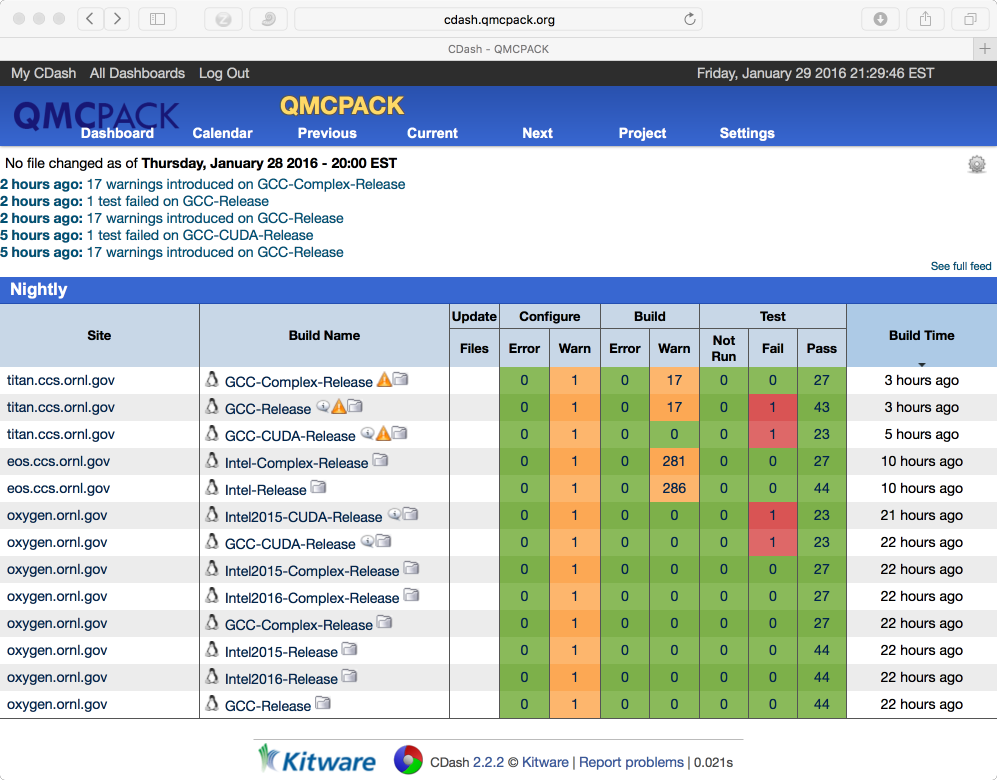
\includegraphics[width=10cm]{figures/QMCPACK_CDash_CTest_Results_20160129.png}
  \caption{Example test results for QMCPACK, showing data for a
    workstation (Intel, GCC, both CPU and GPU builds) and for two ORNL
    supercomputers. In this example, 4 errors were found. This
    dashboard is not yet openly accessible, but the developers hope
    to make it available at a later date.}
  \label{fig:cdash}
\end{figure}

\section{Building ppconvert, a pseudopotential format converter}
\label{sec:buildppconvert}
QMCPACK includes a utility, ppconvert, to convert between different
pseudopotential formats. Examples include effective core potential
formats (in gaussians), the UPF format used by Quantum ESPRESSO, and
the XML format used by QMCPACK itself. The utility also enables the
atomic orbitals to recomputed via a numerical density functional
calculation if they need to be reconstructed for use in an
electronic structure calculation.

To build ppconvert follow the instructions in
src/QMCTools/ppconvert/README. Currently ppconvert is not built
automatically although we expect to automate it soon. The makefile
must be updated to refer to suitable C++ compiler and link in
BLAS. Due to the small size of the calculations, optimal settings are
not essential.

\section{Installing and patching Quantum ESPRESSO}
\label{sec:buildqe}
For trial wavefunctions obtained in a plane-wave basis we mainly
support Quantum ESPRESSO. Note that ABINIT and QBox were supported historically
and could be reactivated.

Quantum ESPRESSO currently stores wavefunctions in a non-standard internal
``save'' format. To convert these to a conventional HDF5 format file
we have developed a converter, pw2qmcpack. This is an add on to the
Quantum ESPRESSO distribution.

To simplify the process of patching Quantum ESPRESSO we have developed
a script that will automatically download and patch the source
code. The patches are specific to each version. e.g. To download and
patch QE v5.3.0:
\begin{verbatim}
cd external_codes/quantum_espresso
./download_and_patch_qe5.3.0.sh
\end{verbatim}
After running the patch, you must configure Quantum ESPRESSO with
the HDF5 capability enabled, i.e.
\begin{verbatim}
cd espresso-5.3.0
./configure --with-hdf5 HDF5_DIR=/opt/local   # Specify HDF5 base directory
\end{verbatim}

The complete process is described in external\_codes/quantum\_espresso/README.

The tests involving pw.x and pw2qmcpack.x have been integrated in the test suite of QMCPACK.
By adding \texttt{-D QE\_BIN=your\_QE\_binary\_path} in the cmake command line when building your QMCPACK,
tests named with ``qe-'' prefix will be included in the test set of your build.
You can test the whole pw$\to$pw2qmcpack$\to$qmcpack workflow by
\begin{verbatim}
ctest -R qe
\end{verbatim}
See Sec.\ref{sec:integtestqe} and the testing section for more details.

\section{How to build the fastest executable version of QMCPACK}
\label{sec:buildperformance}
To build the fastest version of QMCPACK we recommend the following:
\begin{itemize}
\item Use the latest C++ compilers available for your
  system. Substantial gains have been made optimizing C++ in recent
  years.
\item Use a vendor optimized BLAS library such as Intel MKL and AMD ACML. Although
  QMC does not make extensive use of linear algebra, it is used in the
  VMC wavefunction optimizer, to apply the orbital coefficients in local basis
  calculations, and in the Slater determinant update.
\item Use a vector math library such as Intel VML.  For periodic
  calculations, the calculation of the structure factor and Ewald
  potential benefit from vectorized evaluation of sin and
  cos. Currently we only autodetect Intel VML, as provided with MKL,
  but support for MASSV and AMD LibM is included via \#defines. See,
  e.g. src/Numerics/e2iphi.h. For
  large supercells, this optimization can gain 10\% in performance.
\end{itemize}

Note that greater speedups of QMC calculations can usually be obtained by
carefully choosing the required statistics for each
investigation. i.e. Do not compute smaller error bars than necessary.

\section{Troubleshooting the installation}
\label{sec:troubleshoot}
Some tips to help troubleshoot installations of QMCPACK:
\begin{itemize}
\item First, build QMCPACK on a workstation that you control, or on any
  system that has a simple and up-to-date set of development
  tools. You can compare the results of cmake and QMCPACK on this
  system with any more difficult systems you encounter.
\item Use up to date development software, particularly a recent
  CMake. 
\item Verify that the compilers and libraries that you expect are
  being configured. It is common to have multiple versions
  installed. The configure system will stop at the first version it
  finds which might not be the most recent. If this occurs, specify the appropriate
  directories and files directly (Section
  \ref{sec:cmakeoptions}). e.g. cmake -DCMAKE\_C\_COMPILER=/full/path/to/mpicc -DCMAKE\_CXX\_COMPILER=/full/path/to/mpicxx ..
\item To monitor the compiler and linker settings, use a verbose build, ``make
  VERBOSE=1''. If an individual source file fails to compile you
  can experiment by hand using the output of the verbose build to
  reconstruct the full compilation line.
\end{itemize}

If you still have problems please post to the QMCPACK Google group with full
details, or contact a developer.
